\section{Přesnost lokalizace}
\label{sec:Chapter62}

Jako obecná metrika výkonu našich modelů jako celku může být zvolena jako aritmetický průměr chyby se směrodatnou odchylkou, kterou vidíme v následující tabulce:
\begin{table}[H]
    \centering
    \begin{tabular}{lrr}
        \toprule
        Model & Průměrná chyba $\pm$ směrodatná odchylka & Variační koeficient \\
        \midrule
        U-Net & 0.769738 $\pm$ 1.327877 & 1.725102 \\
        U-Net++ bez HS & 0.691072 $\pm$ 1.201024 & 1.737914 \\
        U-Net++ s HS & 0.817158 $\pm$ 1.349039 & 1.650890 \\
        U-Net STN 3-parametrový & 1.024144 $\pm$ 1.075344 & 1.049993 \\
        U-Net STN 6-parametrový & 1.056580 $\pm$ 1.080963 & 1.023078 \\
        \bottomrule   
    \end{tabular}
    \caption[Průměrná chyba a směrodatná odchylka trénovaných modelů]{Průměrná chyba a směrodatná odchylka trénovaných modelů mezi všemi kanály. Jednotka je Euklidová vzdálenost v pixelech na 128$\times$128 snímcích.}
    \label{fig:mean_std_no_channel}
\end{table}

V tabulce \ref{fig:mean_std_no_channel} můžeme vidět srovnanou průměrnou chybu lokalizace sítí. Původní model \textbf{U-Net} dosahuje na testovacím datasetu poměrně dobrých výsledků. 

Model \textbf{U-Net++} se avšak zřetelně neodlišil procentuálně, jak bylo původně na základě rešerše očekáváno (literatura \cite{unetpp} a \cite{unet_comparison}). Dokonce verze s hlubokou supervizí dosáhla horších výsledků, než původní síť U-Net. Verze s HS a průměrným výstupem ze všech 4 výstupních větví (jak specifikováno v orig. lit. \cite{unetpp}) dosáhla až detrimentálních výsledků:
\begin{table}[H]
    \centering
    \begin{tabular}{lrr}
        \toprule
        Model & Průměrná chyba $\pm$ směrodatná odchylka & Variační koeficient \\
        \midrule
        U-Net++ s HS a průměrem výstupů & 1.104677 $\pm$ 2.007999 & 1.817725 \\
    \end{tabular}
    \caption[Průměrná chyba a směrodatná odchylka modelu původní sítě U-Net++ s HS]{Průměrná chyba a směrodatná odchylka modelu U-Net++ s HS a průměrovanou výstupní mapou.}
    \label{fig:mean_std_no_channel_unetpp_fail}
\end{table}

Verze \textbf{bez hluboké supervize} dosáhla zlepšení, avšak může být argumentováno, že primárním důvodem je zvětšení počtu parametrů a velikosti sítě. Jedním z pravděpodobných důvodů neuplatnění slíbeného potenciálu sítí U-Net++ může být úloha samotná, jelikož ve dvou zmíněných literaturách se nejedná o lokalizaci, avšak segmentaci.

Verze modelů \textbf{s modulem STN} avšak dosáhla význameného zlepšení. Variační koeficient a směrodatná odchylka je významně nižší, než u původního modelu sítě U-Net. I když U-Net STN dosahuje vyšších průměrných chyb, je zřetelné, že obecný výkon sítě daleko více převažuje možnosti sítí U-Net a U-Net++ v úlohách lokalizace v rámci této práce. Tento úsudek může být dokázán na vizualizaci průměrné chyby lokalizace v následujícím grafu \ref{fig:loc_distance}:
\pagebreak
\begin{figure}[ht]
\centering
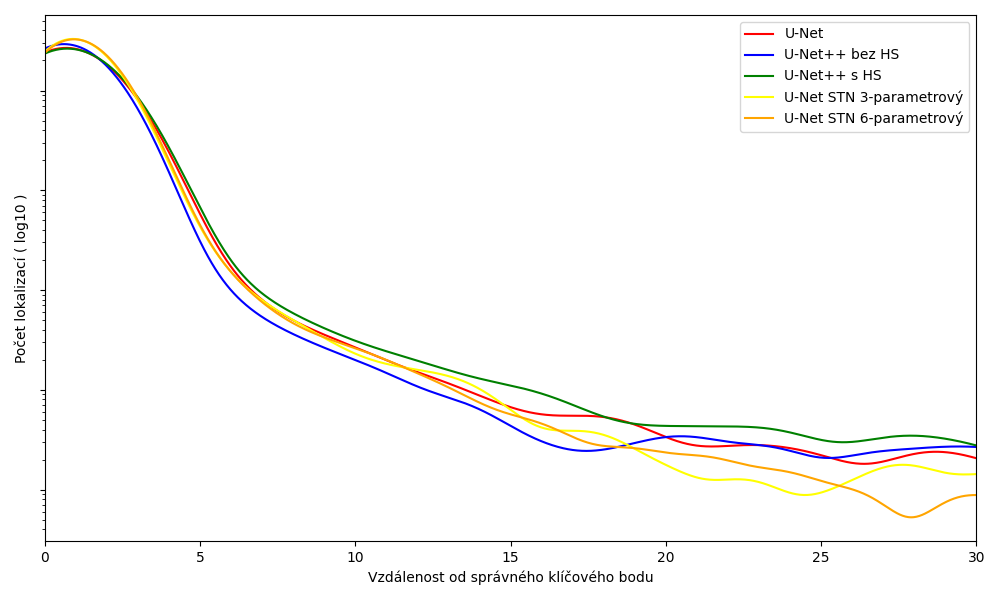
\includegraphics[width=0.8\textwidth,keepaspectratio]{Figures/plots/loc_distance.png}
\caption[Chyba lokalizace modelů]{Chyba lokalizace zobrazená pomocí KDE v logaritmickém měřítku. }
\label{fig:loc_distance}
\end{figure}

Obdobně vykazují podobné rozdíly mezi modely i síla lokalizace (maximální hodnota na výstupním kanále sítě v bodě lokalizace) v následujícím grafu \ref{fig:loc_strength}:

\begin{figure}[H]
\centering
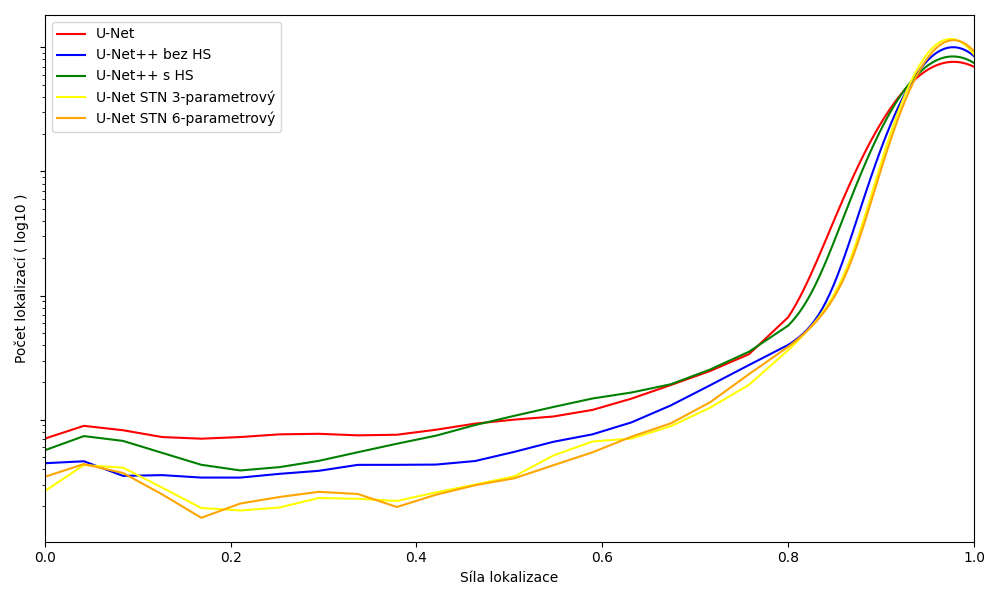
\includegraphics[width=0.8\textwidth,keepaspectratio]{Figures/plots/loc_strength.png}
\caption[Síla lokalizace modelů]{Síla lokalizace zobrazena pomocí KDE v logaritmickém měřítku. }
\label{fig:loc_strength}
\end{figure}

Kompletní a obsáhlý přehled výsledků lokalizace také i mezi kanály může být vidět v tabulce \ref{tab:mean_std_channels}:

\begin{table}[ht]
    \centering
    \begin{tabular}{llllll}
    \toprule
    Kanál & U-Net & U-Net++ bez HS & U-Net++ s HS & U-Net STN 3p & U-Net STN 6p \\
    \midrule
    0 & 1.5$\pm$0.81 & 0.79$\pm$0.66 & 1.18$\pm$0.84 & 0.94$\pm$1.07 & 0.84$\pm$1.08 \\
    1 & 0.73$\pm$0.78 & 0.74$\pm$0.65 & 0.74$\pm$0.83 & 0.69$\pm$1.0 & 0.68$\pm$1.04 \\
    2 & 1.84$\pm$0.94 & 0.98$\pm$0.84 & 1.46$\pm$0.99 & 1.0$\pm$1.17 & 1.52$\pm$1.21 \\
    3 & 1.85$\pm$1.0 & 1.79$\pm$0.99 & 2.08$\pm$1.13 & 1.8$\pm$1.29 & 1.47$\pm$1.27 \\
    4 & 0.96$\pm$0.6 & 1.21$\pm$0.53 & 1.02$\pm$0.66 & 1.03$\pm$0.88 & 0.97$\pm$0.93 \\
    5 & 0.67$\pm$0.59 & 0.58$\pm$0.46 & 0.69$\pm$0.55 & 0.7$\pm$0.82 & 0.49$\pm$0.8 \\
    6 & 0.95$\pm$0.69 & 1.24$\pm$0.64 & 1.28$\pm$0.81 & 0.62$\pm$0.96 & 0.68$\pm$1.03 \\
    7 & 1.16$\pm$0.83 & 1.13$\pm$0.74 & 1.35$\pm$0.84 & 0.77$\pm$1.05 & 0.7$\pm$1.13 \\
    8 & 0.62$\pm$0.52 & 0.72$\pm$0.55 & 0.8$\pm$0.49 & 0.42$\pm$0.79 & 0.43$\pm$0.82 \\
    9 & 0.97$\pm$0.85 & 1.06$\pm$0.76 & 1.07$\pm$0.88 & 0.89$\pm$1.13 & 0.9$\pm$1.17 \\
    10 & 2.17$\pm$0.85 & 2.03$\pm$0.81 & 2.16$\pm$0.99 & 1.86$\pm$1.12 & 1.97$\pm$1.16 \\
    \bottomrule
    \end{tabular}
    \caption[Průměr a směrodatná odchylka vzdálenosti mezi kanály a sítěmi]{Průměr a směrodatná odchylka vzdálenosti lokalizace mezi kanály a sítěmi.}
    \label{tab:mean_std_channels}
\end{table}


\endinput